\documentclass[12pt, letterpaper]{article}

%-------Packages---------
\usepackage{amssymb,amsfonts}
\usepackage{mathptmx}
\usepackage{amsthm}
\usepackage{graphicx}
\usepackage[all,arc]{xy}
\usepackage[colorlinks=true, allcolors=blue]{hyperref}
\usepackage{enumerate}
\usepackage{bbm}
\usepackage{dsfont}
\usepackage{mathrsfs}
\usepackage{tikz-cd}
\usepackage{setspace}
\usepackage{import}
\usepackage[utf8]{inputenc}
\usepackage{hyperref}
\usepackage{tikz}
\usepackage{float}
\usepackage{mdframed}
\usepackage{fancyhdr}
\usepackage[nointegrals]{wasysym}

\usepackage[left=1in,top=1in,right=1in,bottom=1in]{geometry}

\usepackage{mathtools}
\usepackage{setspace}
\usepackage{cleveref}
\usepackage{multicol}

%--------Theorem Environments--------
%theoremstyle{plain} --- default
\newmdtheoremenv{theorem}{Theorem}[subsection]
\newmdtheoremenv{corollary}[theorem]{Corollary}
\newtheorem{proposition}[theorem]{Proposition}
\newmdtheoremenv{lemma}[theorem]{Lemma}
\newtheorem{conj}[theorem]{Conjecture}
\newtheorem{quest}[theorem]{Question}

\theoremstyle{definition}
\newmdtheoremenv{definition}[theorem]{Definition}
\newmdtheoremenv{definitions}[theorem]{Definitions}
\newtheorem{example}[theorem]{Example}
\newtheorem{algorithm}[theorem]{Algorithm}
\newtheorem{rmk}[theorem]{Remark}
\newtheorem{exercise}[theorem]{Exercise}

%----------- my commands -------------
\newcommand{\C}{\mathbb{C}}
\newcommand{\R}{\mathbb{R}}
\newcommand{\Q}{\mathbb{Q}}
\newcommand{\Z}{\mathbb{Z}}
\newcommand{\N}{\mathbb{N}}
\renewcommand{\P}{\mathbb{P}}
\newcommand{\contr}{\Rightarrow \Leftarrow}
\newcommand{\HRule}[1]{\rule{\linewidth}{#1}}
\newcommand{\s}{\(\,\)}
\renewcommand{\t}[1]{\text{#1}}
\newcommand{\ang}[1]{\left\langle #1 \right\rangle}

% Meta data
\setstretch{1.2}

\begin{document}

\pagestyle{fancy}
\fancyhf{}
\fancyhead[LOE]{\slshape{\textbf{Vincent Ferrara}}}
\fancyhead[ROE]{\thepage}

\subsection*{Problem 1}
By Lagrange's Theorem we know that $S_4$ has subgroups of order $1,2,3,4,6,8,12$\\
Let $H$ be a subgroup of order $12$. By Cauchy's Theorem we know it has a subgroup of order $3$. Thus, it has a 3 cycle.
Since it has a 3 cycle we know it is $A_4$ since $A_4$ is generated by 3 cycles, and this is normal since it has index 2.\\
Let $H$ be a group of order $8$. These must be $2$-Sylow subgroups and by Sylow 3 we know there is 1 or 3 but there is 3 since two examples are $\ang{(1234),(13)}$ and $\ang{(1243),(14)}$
Thus these are all conjugate by Sylow 2 thus these are not normal.\\
Let $H$ be a group of order 6. This must be $S_3$ since there is no elements of order $6$ in $S_4$. This means it has a $3$ cycle but since all $3$ cycles are conjugate we know that we can get an
element outside the subgroup since the $S_3$ subgroup will only have 2 3-cycles.\\
Let $H$ be a group of order 4. This is either $C_4$ or $C_2 \times C_2$. If it is $C_4$ then it is a cycle group generated by a 4 cycle, and since $\sigma(abcd)\sigma^{-1}=(\sigma(a)\sigma(b)\sigma(c)\sigma(d))$ we know that all $4$ cycles 
are conjugate. Thus, since there 6 4-cycles we know we can get ouside our group of 4.\\
If it is $C_2\times C_2$ then if it has a transposition then we can get out again by similar proof by showing all transpositions are conjugate. Thus the only possibility is $\ang{(12)(34),(13)(24)}$\\
Since these aree a product of disjoint cycles if we conjugate $\sigma(ab)(cd)\sigma^{-1}=(\sigma(a)\sigma(b))(\sigma(c)\sigma(d))$ then since $\sigma$ permutes elements we know that this will also result in a prodcuut of disjoint transpositions and we have them all in this subgroup this is normal.\\
Let $H$ be a group of order 3. Similar to order 4 for $C_4$ this is not normal\\
Let $H$ be a group of order 2. SImilarr to order 4 for $C_4$ this is not normal\\
Thus we only have normal groups $\ang{(12)(34),(13)(24)}$, $A_4$ and $\{e\}$\\
For normal in $A_4$ we know from previous homework that it has normal $C_2\times C_2$ and this could only be $\ang{(12)(34),(13)(24)}$\\
Thus all composition series are\\
$S_4 \unrhd A_4 \unrhd \ang{(12)(34),(13)(24)} \unrhd \{1, (12)(34)\} \unrhd \{e\}$\\
$S_4 \unrhd A_4 \unrhd \ang{(12)(34),(13)(24)} \unrhd \{1, (13)(24)\} \unrhd \{e\}$\\
$S_4 \unrhd A_4 \unrhd \ang{(12)(34),(13)(24)} \unrhd \{1, (14)(23)\} \unrhd \{e\}$

\newpage
\subsection*{Problem 2}
\begin{enumerate}[(a)]
    \item For $A_4$, Consider the homomorphism $\varphi : A_4 \rightarrow A_4 \diagup \ang{(12)(34),(13)(24)}$ since $|\ang{(12)(34),(13)(24)}|=4$ and is normal we know $A_4 \diagup \ang{(12)(34),(13)(24)} \cong C_3$ which is abelian.\\
    Consider $[a,b] \in A_4'$, $aba^{-1}b^{-1}$. $\varphi(aba^{-1}b^{-1})=\varphi(a)\varphi(b)\varphi(a)^{-1}\varphi(b)^{-1}=e$ since it is abelian thus $A_4' \in \t{ker}(A_4 \diagup \ang{(12)(34),(13)(24)})$ and the kernel of this is $\ang{(12)(34),(13)(24)}$ thus $A_4' \leq \ang{(12)(34),(13)(24)}$\\
    Consider $(123)(12)(34)(132)(12)(34)=(13)(24)$, $(124)(12)(34)(142)(12)(34)=(14)(23)$, and $(13)(24)(14)(23)=(12)(34)$ thus we know $A_4' = \ang{(12)(34),(13)(24)}$ and since $\ang{(12)(34),(13)(24)}$ is abelian $\ang{(12)(34),(13)(24)}'=\{e\}$\\
    Thus it is solvable and the derived series is $A_4 \unrhd \ang{(12)(34),(13)(24)} \unrhd \{e\}$\\
    For $C_{12}$ since it is abelian its derived serries is $C_{12} \unrhd \{e\}$ thus it is solvable\\
    For $D_6$ we know it has a normal subgroup $\ang{x^2}$ thus we know $D_6 \diagup \ang{x_2}$ is a group of order 4 which we know is abelian thus from similar proof to above we know $D_6' \leq \ang{x^2}$\\
    Consider $yx^2y^{-1}x^{4}=x^{8}=x^{2}$ thus $D_6' = \ang{x^2}$ and since $\ang{x^2}$ is abelian its commutator subgroup is $\{e\}$ thus it is solvable\\
    $D_6 \unlhd \ang{x^2} \unlhd \{e\}$\\
    For $C_6 \times C_2$ it is abelian thus $C_6 \times C_2 \unrhd \{e\}$ and it is solvable\\
    For $C_3 \rtimes C_4$ we know it has a normal subgroup $C_3$ thus $(C_3 \rtimes C_4) \diagdown C_3$ is order 4 and thus abelian thus $(C_3 \rtimes C_4)' \leq C_3$\\
    Consider $bab^{-1}a^2=a^4=a$ thus $C_3 = (C_3 \rtimes C_4)'$ and since $C_3$ is abelian, $C_3'=\{e\}$\\
    Thus it is solvable with $C_3 \rtimes C_4 \unrhd C_3 \unrhd \{e\}$
    \item \begin{itemize}
        \item For $n=1$, $S_1=\{e\}$ thus done, and it is solvable
        \item For $n=2$, $S_2 \cong C_2$ thus it is abelian thus $S_2 \unlhd \{e\}$, and thus solvable
        \item For $n=3$, $S_3 \cong D_3$ thus it has a normal subgroup $C_3$ and since $D_3 \diagup C_3 \cong C_2$ it is abelian thus $D_3' \leq C_3$\\
        Consider $yxy^{-1}x^2=x^4=x$ thus $C_3 \leq D_3'$ thus $D_3' = C_3$ thus since it is abelian $C_3'=\{e\}$ thus it is solvable with $S_3=D_3 \unrhd C_3 \unrhd \{e\}$
        \item For $n=4$, we know $S_4$ has normal subgroup $A_4$ thus $S_4 \diagup A_4 \cong C_2$ thus abelian thus $S_4' \leq A_4$\\
        Consider $(14)(123)(14)(132)=(142)$ thus since $S_4'$ is normal we can conjugate this 3-Cycle to get all 3-Cycles and thus $S_4'=A_4$ and for $A_4$ look above thus it is solvable\\
        $S_4 \unrhd A_4 \unrhd \dots$
        \item For $n\geq5$ by similar proof above we can show that $S_n'=A_n$ and since $A_n$ is simple we know that $A_n'=\{e\}$ or $A_n$ if it is $\{e\}$ this would mean it is abelian which is not true thus it is $A_n$ thus the
        derived series is $S_n \unrhd A_n \unrhd A_n \cdots$ thus not solvable
    \end{itemize}
\end{enumerate}

\newpage
\subsection*{Problem 3}
\begin{tabular}{c|ccc|c|ccccccccccc|c|ccccccc|c}
      & $y$ &   & $y$ &   & $x$ &   & $x$ &   & $x$ &   & $\cdots$ &   & $x$ &   & $x$ &   & $x$ &   & $y$ &   & $x$ &   & $y$ & \\
    1 &     & 1 &     & 1 &     & 2 &     & 3 &     & 4 & $\cdots$ &   &     &$n$&     & 1 &     & 2 &     &$n$&     & 1 &     & 1\\
    2 &     &$n$&     & 2 &     & 3 &     & 4 &     & 5 & $\cdots$ &   &     & 1 &     & 2 &     & 3 &     &$n-1$&   &$n$&     & 2\\
    3 &     &$n-1$&   & 3 &     & 4 &     & 5 &     & 6 & $\cdots$ &   &     & 2 &     & 3 &     & 2 &     &$n-2$&   &$n-1$&   & 3\\
$\vdots$&&$\vdots$&&$\vdots$&&$\vdots$&&$\vdots$&&$\vdots$& $\cdots$ & &     &$\vdots$&     &$\vdots$&     &$\vdots$&     &$\vdots$&     &$\vdots$&     &$\vdots$\\
   $n$&     & 2 &     &$n$&     & 1 &     & 2 &     & 3 & $\cdots$ &   &     &$n-1$&   &$n$&     & 1 &     & 1 &     & 2 &     &$n$\\
\end{tabular}
Thus we know since $1=\{y\}$ is index $n$ and does not act trivially we know $G$ has order $2n$

\newpage
\subsection*{Problem 4}
\begin{align*}
    x^2&=yxy\\
 x^2y^2&=yx\\
   \phantom{text}\\
  x^4=e&=yxyyxy\\
      e&=x^2y^3xy\\
      e&=x^3y\\
      x&=y
\end{align*}
Thus the order of $x$ and $y$ both divide 3,4 thus they have order 1 thus $x=y=e$\\
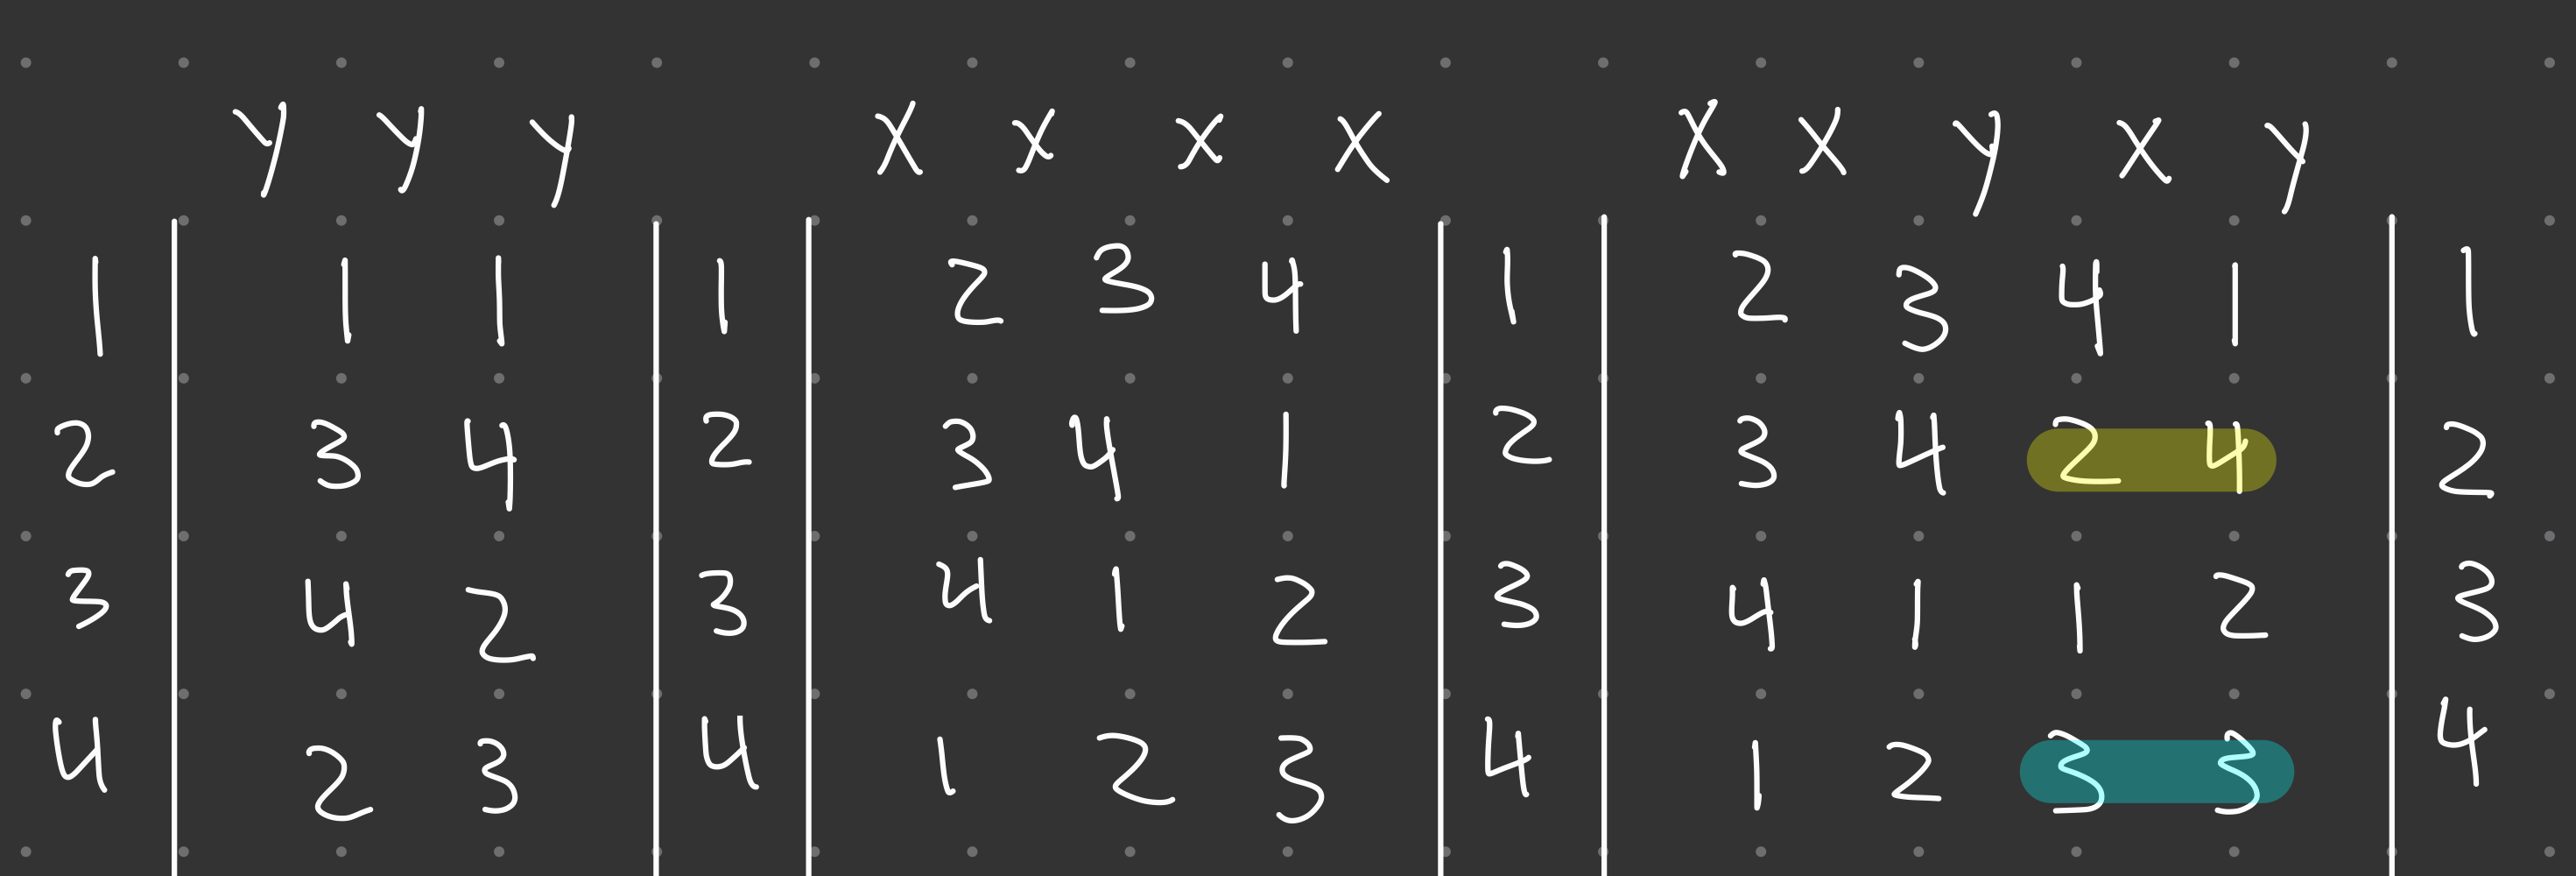
\includegraphics[scale=0.15]{table1.png}\\
We can see from the table that from the yellow $2=3$, from the blue $4=2$\\
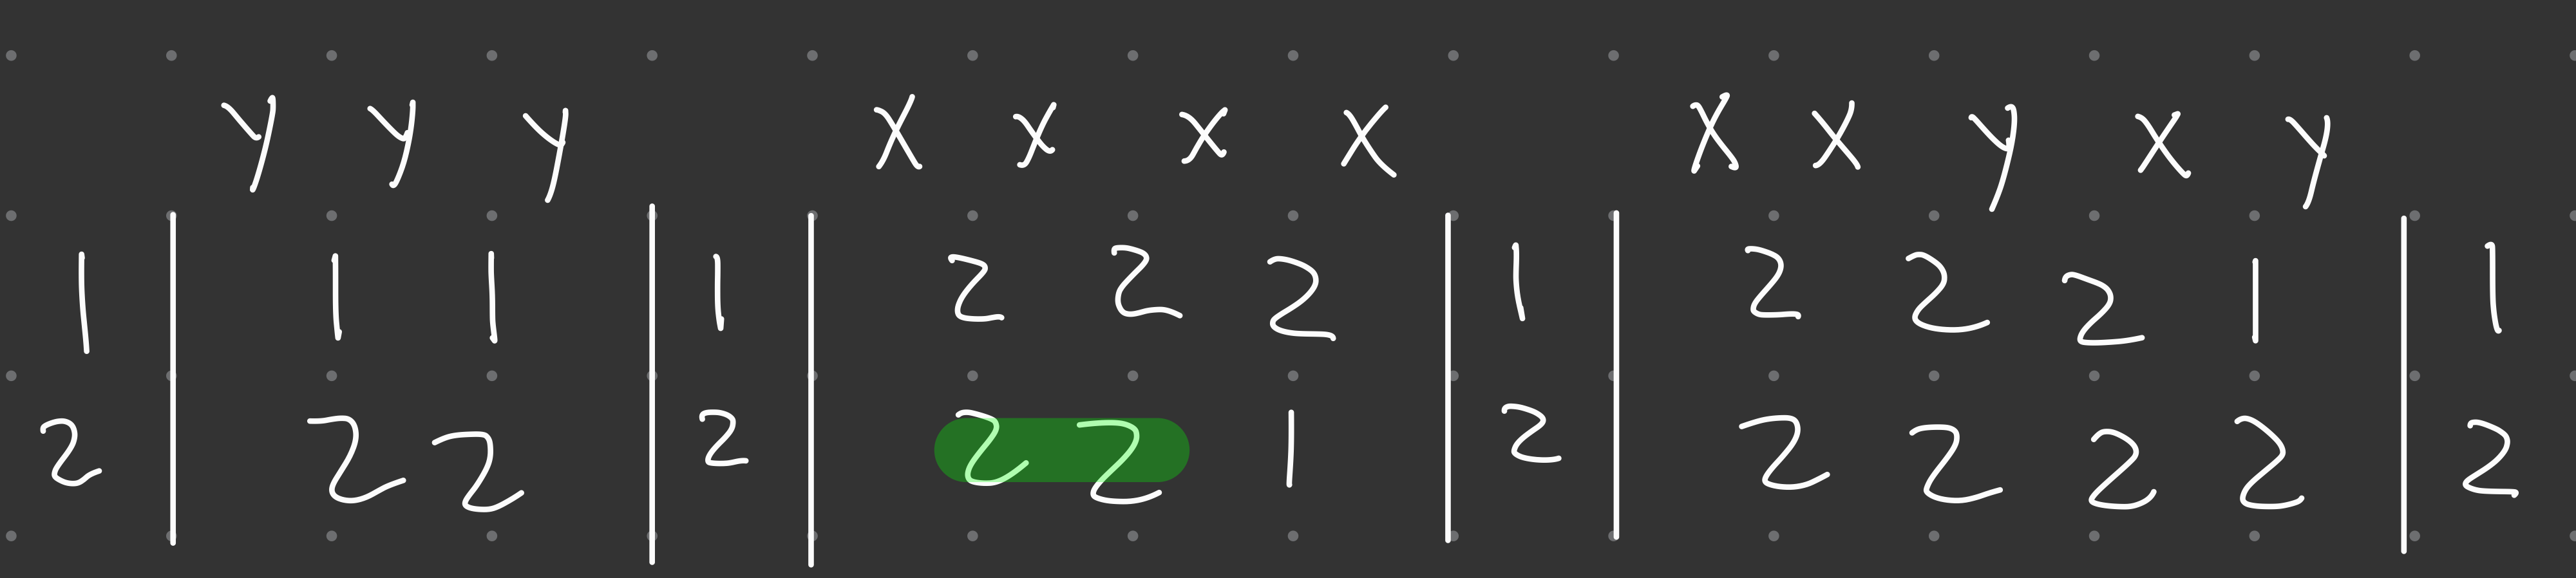
\includegraphics[scale=0.11]{table2.png}\\
We can see from the green that $2=1$ thus this is a trivial table thus $x=y=e$

\newpage
\subsection*{Problem 5}
\begin{enumerate}[(a)]
    \item 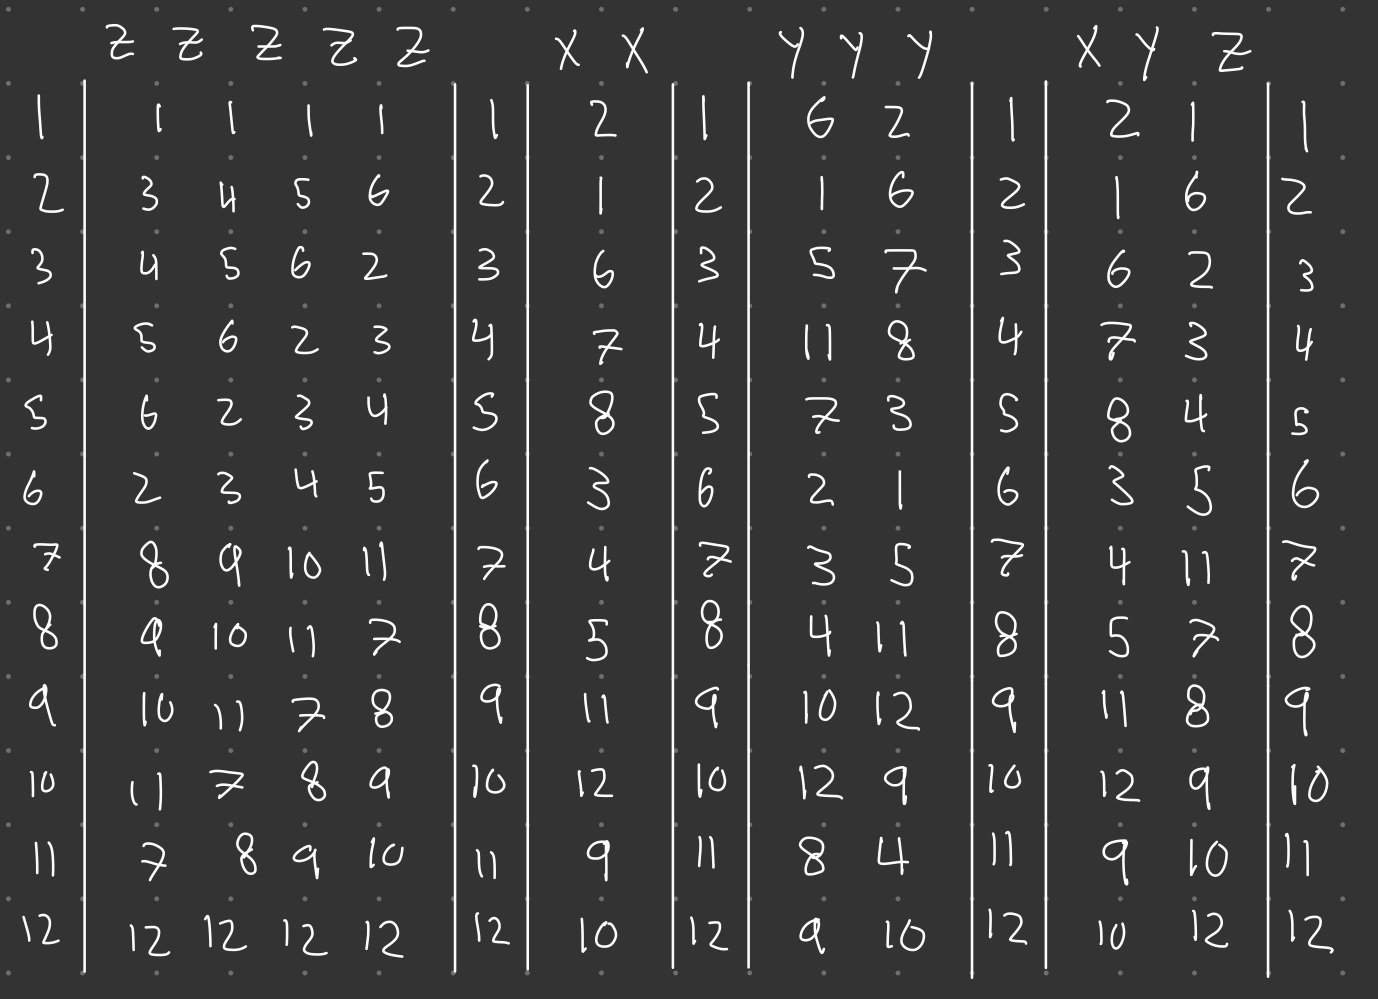
\includegraphics[scale=0.25]{table.png}\\
    Since $z$ does not act trivially we know that $[G: \ang{z}]=12$ thus $|G|=60$
    \item From the table above since all of the elementts do not act trivially we know since they divide a prime order they must be that prime order so $z$ is order 5, $x$ is order 2, and $y$ is order 3.\\
    Consider $z=y^2x$ thus we can rewrite $G$ to be $G=\ang{x,y \mid x^2=y^3=(y^2x)^5=e}$\\
    Let $\varphi: G \rightarrow A_5$ s.t. $\varphi(x)=(12)(34)$, and $\varphi(y)=(235)$\\
    Homomorphism:\\
    We only have to check $(\varphi(y)^2\varphi(x))^5=e$\\
    $((253)(12)(34))^5=e$ thus this is a homomorphism\\
    Injective: Let $a \in \t{ker}(\varphi)$\\
    If $\varphi(a)=\varphi(x^iy^j)=\varphi(x)^i\varphi(y)^j=((12)(34))^i(235)^j=e$\\
    If $i$ is even then $=(234)^j=e$ thus $j$ is a multiple of 3 thus $a=e$\\
    If $j$ is odd then $=(12)(34)(235)^j=e$\\
    If $j$ is a multiple of 3 then $(12)(34)=e$ which is not possible so\\
    either $=(12)(34)(235)$ or $=(12)(34)(253)$\\
    If the first case then $(12)(34)(235)=e$ this is not possible\\
    If the second case then $(12)(34)(253)=e$ this is not possible\\
    If $\varphi(a)=\varphi(y^jx^i)=\varphi(y)^j\varphi(x)^i=(235)^j((12)(34))^j=e$\\
    Similar proof as above.
    Thus, $a=e$\\
    Thus injective\\
    Thus since $|G|=|A_5|$ and $\varphi$ is injective $\varphi$ is bijective thus $G \cong A_5$\\
    Thus consider $H$ use $\varphi$, and we get that $\varphi(H)\leq A_5$ call this subgroup $K$\\
    Consider $K$, it is generated by $\varphi(y^2xyxy)=(142)$ and $\varphi(x)=(12)(34)$\\
    Since $K$ is generated by even permutations with only 4 elements we know that $K \leq A_4$\\
    We know $K$ has at least $5$ elements $\{e,(142),(124),(12)(34),(142)(12)(34)=(243)\}$ thus $|K|=12$ since if $|K|=6$ then since $G$ has no
    element of order $6$ is must be $S_3$ and $S_3$ has 3 elements of order 2 thus $K$ must have 3 double transpositions but theese form a subroup of order 4 but 4 does not divide 6 thus
    $|K|=12$
    Thus $G$ acts on $G \diagup H$ by left multiplying on $H$'s $[G:H]=5$ cosets thus $\phi: G \rightarrow S_5$\\
    $H \cong K \cong A_4$
    \item I did that above
    \item Consider $K$ use $\varphi$, and we get that $\varphi(K) \leq A_5$ call this subgroup $B$\\
    Consider $B$, it is generated by $\varphi(yxy^2x)=(15234)$ and $\varphi(x)=(12)(34)$\\
    $(15234)$ is order 5, and $(12)(34)$ is order 2.\\
    Consider $(12)(34)(15234)(12)(34)=(14325)=(15234)^{-1}$ thus $B \cong D_5$\\
    Thus $K \cong B \cong D_5$ thus $|K|=10$\\
    Thus $G$ acts on $G \diagup K$ by left multiplying on $K$'s $[G:K]=6$ cosets thus $\phi: G \rightarrow S_6$\\
\end{enumerate}

\newpage
\subsection*{Problem 6}
\begin{enumerate}[(a)]
    \item Consider $(xyx^{-1}y^{-1}R)=R$ this is true since $[x,y] \in R$\\
    Since $R$ is normal $xRyR=yRxR$\\
    Thus $x^2Ry^2R=xRyRxRyR=y^2Rx^2R \implies [x^2,y^2]R=R$ thus $[x^2,y^2] \in R$
    \item Consider $c=[x,y]$ this is an element of $F'$ by definition.\\
    Since $F'$ is normal it also has all conjugates of $c$, thus $R \subseteq F'$ since $R$ is the smallest normal group with $c$.\\
    Shown in (a) since the two generators of $F$ commute in $F \diagup R$ we know that $F \diagup R$ is abelian.\\
    Thus shown in problem 2 we know that $F' \leq R$ thus $F' = R$
\end{enumerate}
\end{document}